\documentclass[aps,twocolumn,prl,showpacs,showkeys,preprintnumbers,superscriptaddress,nobibnotes,floatfix,longbibliography,notitlepage,nofootinbib]{revtex4-2}

\usepackage{graphicx}
\usepackage{epstopdf}
\usepackage{amsmath}
\usepackage{amsfonts}
\usepackage{amssymb}
\usepackage{appendix}
\usepackage{enumerate}
\usepackage{natbib}
\usepackage{comment}
\usepackage{bbold}
\usepackage[shortlabels]{enumitem}
\usepackage{color}
\usepackage{slashed}
\usepackage{subfigure}
\usepackage{setspace}
\usepackage{footnote}
\usepackage{lipsum}
\usepackage{multirow}
%\usepackage{longtable}
\usepackage[colorlinks = true,
            linkcolor = blue,
            urlcolor  = blue,
            citecolor = blue,
            anchorcolor = blue]{hyperref}
\usepackage[capitalize]{cleveref}
\usepackage{braket}
\usepackage{multirow}
\usepackage{physics}
\usepackage[normalem]{ulem}
\usepackage{url}
\usepackage{units}
\usepackage[normalem]{ulem}
\usepackage{graphicx}% Include figure files
\usepackage{dcolumn}% Align table columns on decimal point
\usepackage{bm}% bold math
\usepackage{lipsum}
\usepackage{lettrine}

\begin{document}


\preprint{USTC-ICTS/PCFT-24-07}
\bibliographystyle{apsrev4-1}
\title{
Supernovae Time Profiles as a Probe of New Physics at Neutrino Telescopes
}

\author{Jeff Lazar}
\email{jlazar@icecube.wisc.edu}
\affiliation{Department of Physics \& Laboratory for Particle Physics and Cosmology, Harvard University, Cambridge, MA 02138, USA}
\affiliation{Department of Physics \& Wisconsin IceCube Particle Astrophysics Center, University of Wisconsin-Madison, Madison, WI 53706, USA}
\author{Ying-Ying Li}
\email{yingyingli@ustc.edu.cn}
\affiliation{Peng Huanwu Center for Fundamental Theory, Hefei, Anhui 230026, China}
\affiliation{Interdisciplinary Center for Theoretical Study, University of Science and Technology of China, Hefei, Anhui 230026, China}
\author{Carlos A. Arg\"{u}elles}
\email{carguelles@g.harvard.edu}
\affiliation{Department of Physics \& Laboratory for Particle Physics and Cosmology, Harvard University, Cambridge, MA 02138, USA}
\author{Vedran Brdar}
\email{vedran.brdar@okstate.edu}
\affiliation{Department of Physics, Oklahoma State University, Stillwater, OK, 74078, USA}

%\date{\today}

\begin{abstract}
Neutrino telescopes, including IceCube, can detect galactic supernova events by observing the collective rise in photomultiplier count rates with a sub-second time resolution. 
Leveraging precise timing, we demonstrate the ability of neutrino telescopes to explore new weakly coupled states emitted from supernovae and subsequently decaying to neutrinos.
Our approach utilizes publicly available packages, \texttt{ASTERIA} and \texttt{SNEWPY}, for simulating detector responses and parametrizing neutrino fluxes originating from Standard Model and new physics. 
We present results for two beyond the Standard Model scenarios and introduce the tool developed for testing a diverse range of new physics models.
\end{abstract}

\maketitle

\textbf{\textit{Introduction}}---The Standard Model (SM) is a remarkable but incomplete theory. 
Puzzles such as the non-vanishing neutrino mass, the origin of observed matter-antimatter asymmetry, and the nature of dark matter, among others, seek explanations beyond the SM (BSM).
Since there are also no firmly established clues on the energy scale at which the new particles should appear, numerous BSM searches across a wide range of scales have been performed: from collider searches at high energies~\cite{Nath:2010zj} to studies of cosmic microwave background at temperatures near absolute zero~\cite{Baumann:2015rya}.

Supernovae (SNe) release most of their energy in neutrinos, offering unique opportunities to test BSM physics via neutrino interactions.
The duration of the burst~\cite{Kamiokande-II:1987idp,Bionta:1987qt,Baksan} and inferred total energy of neutrinos~\cite{Loredo:2001rx,Pagliaroli:2008ur,Huedepohl2010} from SN 1987A---the only SN observed in neutrinos---have already given tentative constraints on the energies that could be carried by light BSM particles produced in the interior of a star.
Indeed, many different BSM scenarios have been constrained in this way, see \textit{e.g.} Refs.~\cite{Raffelt:2011nc,Arguelles:2016uwb,Suliga:2020vpz,Lucente:2021hbp,Caputo:2022rca,Caputo:2021rux,PhysRevD.100.083002,DeRocco:2019njg,Kazanas:2014mca,Magill:2018jla}.
If, additionally, BSM particles emitted from SNe can decay to neutrinos en route to Earth, even stronger limits can be set, as shown, for instance, in Ref.~\cite{Fiorillo:2022cdq} for Majoron-like bosons and in Ref.~\cite{Brdar:2023tmi} for a realization featuring a neutrino magnetic moment portal.
In contrast to SM neutrinos, BSM states produced in the SN core can freely stream out without further interactions.
Consequently, they exit with higher energies than neutrinos, typically around $\mathcal{O}(100)$~MeV.
Provided such particles decay to neutrinos, strong constraints can be set from the fact that neutrinos of $\mathcal{O}(100)$~MeV were not recorded from SN 1987A~\cite{Fiorillo:2022cdq, Brdar:2023tmi}.
Such strategies were utilized for neutrino experiments operating during the SN 1987A event. Sensitivity projections for  DUNE~\cite{DUNE:2015lol} and Hyper-Kamiokande~\cite{Hyper-Kamiokande:2018ofw} in light of anticipated galactic SN event were also performed. 

\begin{figure}[t!]
\vspace{0.27cm}
    \centering
    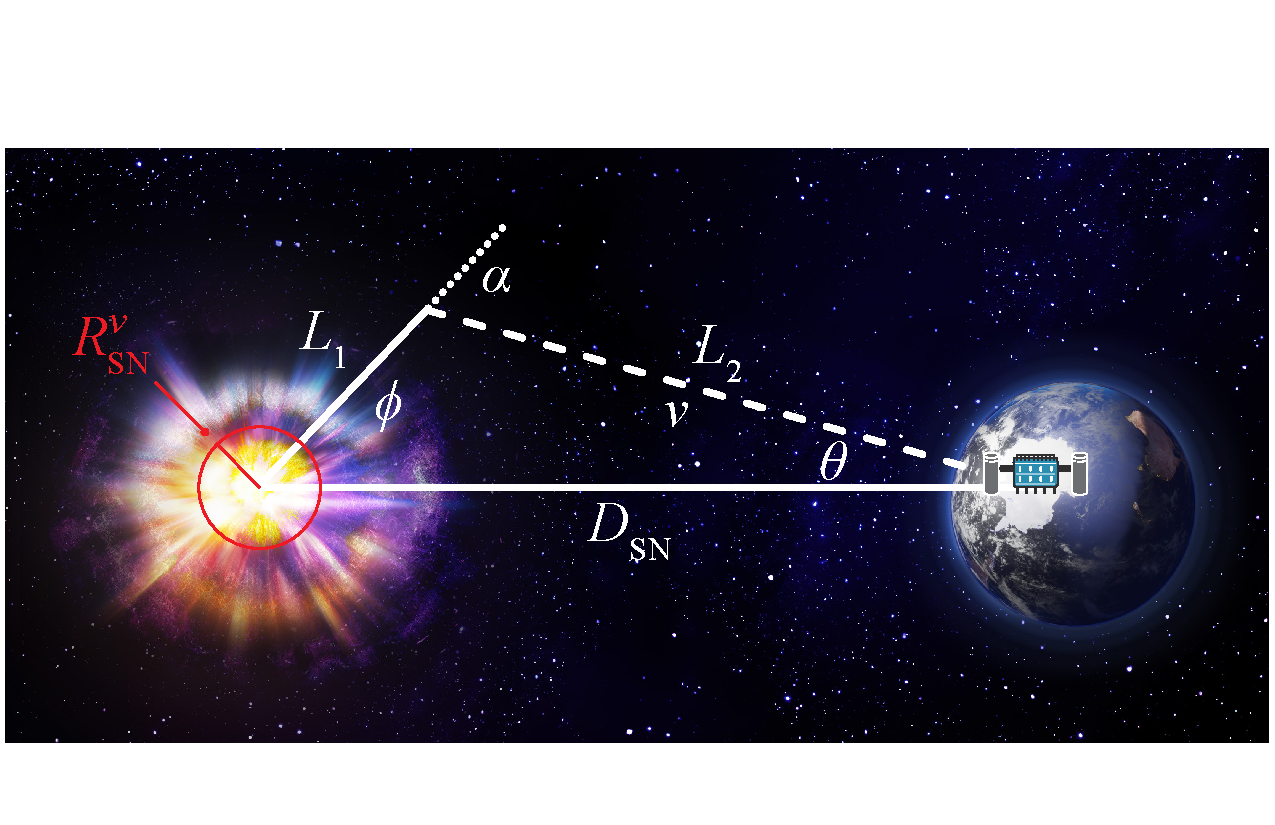
\includegraphics[width=0.48\textwidth]{figures/Supernova_Diagram}
    \caption{\textit{\textbf{The decay geometry for Majorons produced in a SN.}}
    Both the additional distance travelled relative to the direct line of sight and the potential non-relativistic speed of the Majoron can induce a delayed signal relative to the SM signal.
    }
    \label{fig:geometry}
\end{figure}

The IceCube Neutrino Observatory has pioneered the detection of neutrinos at $\mathcal{O}$(PeV) energies~\cite{IceCube:2014stg,IceCube:2018cha} and has identified several specific astrophysical neutrino sources~\cite{IceCube:2018cha,IceCube:2023ame,IceCube:2022der}.
IceCube is also expected to be able to detect the next galactic SN~\cite{Kopke_2011}.
In fact, a search for MeV neutrinos from optically obscured galactic SNe was recently performed in~\cite{IceCube:2023ogt} as well as the search for temporal correlation of MeV neutrino events with fast radio bursts~\cite{IceCube:2019acm}.
In both cases, the observable is a collective rise in all photomultiplier rates on top of the background noise in a certain time window, and it turns out that IceCube is sensitive to intervals as short as $\mathcal{O}(0.01)$ seconds. 
In this Letter, we will demonstrate that such precise time resolution will play a crucial role in testing new physics from SNe.   

BSM states can give rise to off-time signals in two ways.
First, if the BSM particles are non-relativistic, they will produce a delayed signal. 
However, it is also possible that new states are light, implying that they may even exit the SN at earlier times than certain flavors of SM neutrinos.
Such an early BSM signal, which to the best of our knowledge has not been previously considered, can, for instance, be induced by light BSM states produced from $\nu_e$ scattering inside the SN; they would then subsequently decay to $\bar{\nu}_e$, which chiefly induces the signal at IceCube. 
This would happen at early stages of an SN, around the neutralization burst, when $\nu_e$ are present, and $\bar{\nu}_e$ have not been produced yet.
Such novel timing patterns generically exist in models with new weakly interacting particles, such as the aforementioned Majoron model~\cite{Fiorillo:2022cdq} and the neutrino magnetic moment portal~\cite{Magill:2018jla,Brdar:2020quo}.

In this work, we will show that, by using the timing measurements, neutrino telescopes will be able to provide powerful constraints on the BSM parameter space in association with forthcoming galactic SN events.\\
%Via the timing measurement, we will show that neutrino telescopes will be able to provide powerful constraints on the BSM parameter space in association with forthcoming galactic SN events.\\


%%%%%%%%%%%%%%%%%%%%%%%%%%%%%%%%%%%%%%%%%%%%%%%%%%%%%%%%%%%%%%%%%%%%%%%%%%%%%%%%%%%%%%%%%%%%%%%%%%%%%%%%%%%%

\textbf{\textit{The Model}}---First, we consider the Majoron model, studied in Ref.~\cite{Fiorillo:2022cdq}, where SN 1987A constraints were derived.
The relevant part of the Lagrangian reads
\begin{align}
\mathcal{L} \supset -g_{\alpha\beta} \nu_\alpha \nu_\beta \phi + \text{h.c.} - m_\phi \phi\phi^*\,,
\end{align}
where $\phi$ is the (pseudo)scalar, $m_\phi$ is its mass, and $g$ parametrizes interaction strength between $\phi$ and neutrinos.
We assume flavor universal interaction and hence $g_{\alpha\beta}\equiv g_\phi \, \delta_{\alpha\beta}$. 
Majorons are produced from (anti)neutrino coalescence in the star and subsequently decay to a pair of (anti)neutrinos, resulting in BSM (anti)neutrino flux emitted from the star.
The total decay width is given by $\Gamma_\phi = 3g^2 m_\phi/16 \pi$.

We will set SN bounce time $t_{\rm bounce}$ as $t = 0$.
Using data from the simulation of $8.8 M_\odot$ progenitor star~\cite{Huedepohl2010} and including effects of neutrino oscillations assuming normal mass ordering~\cite{Dighe:1999bi}, we calculated standard neutrino fluxes at Earth. Following Ref.~\cite{Fiorillo:2022cdq}, we also calculated the flux of emitted Majorons.
At $t \leq \unit[0.05]{s}$, Majorons are mainly produced through $\nu_e$ and $\nu_x$ coalescence where $\nu_x$ includes (anti)neutrinos of $\tau$ and $\mu$ flavor.
After $\unit[0.05]{s}$, the flux of Majorons decreases with the total flux of neutrinos of all flavors.
Thus, we found that the Majoron flux peaks around $t \sim \unit[0.05]{s}$.
We further cross-checked the agreement with Ref.~\cite{Fiorillo:2022cdq} by reproducing their bound from SN energy loss. 


Very weakly coupled Majorons immediately stream out after being produced inside the star.
On their way to Earth, Majorons of energy $E_\phi$ will travel at the speed of $\beta$ for a distance of $L_1$, then decay to (anti)neutrinos of energy $E_\nu$ at an emission angle $\cos\alpha = (2 E_\phi E_{\nu} - m^2_\phi)/(2E_{\nu}E_\phi\beta)$.
Daughter (anti)neutrinos will travel for a distance $L_2$ and reach Earth at the angle $\theta$ satisfying $D_{\rm SN} \sin\theta = L_1 \sin\alpha$ for a SN that is $D_{\rm SN}$ away; see the decay geometry in \cref{fig:geometry}.
The time delay, $\delta t$, relative to a relativistic particle moving along the line-of-sight path from a SN to reach the Earth is given by~\cite{Jaeckel:2017tud}
\begin{align}
    \delta t = \left(\frac{L_1}{\beta}-L_1\right) + (L_1 + L_2 -D_{\rm SN})\,,
    \label{eq:deltatexa}
\end{align}
where we have split the contribution to $\delta t$ into two parts: the first part comes from the slow-moving Majorons before their decay, and the second part is due to the detour from the line-of-sight path at the given emission angle $\alpha$. 

\begin{figure}[t!]
    \centering
    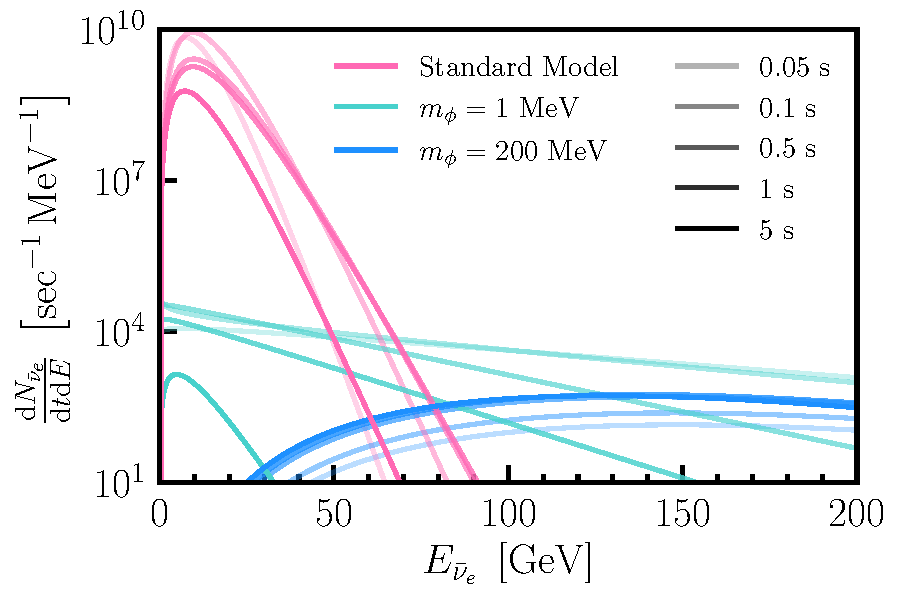
\includegraphics[width=0.47\textwidth]{figures/majoran_fluxes.pdf}
    \caption{\textit{\textbf{Flux of $\bar{\nu}_{e}$ from SM production and two Majoron hypotheses at Earth}}.
    We choose the parameters $g_\phi = 10^{-10.2}$ and $g_\phi = 10^{-11.8}$ for $m_\phi = \unit[1]{MeV}$ and $m_\phi = \unit[200]{MeV}$, respectively.
    }
    \label{fig:fluxes}
\end{figure}

We will consider a SN event that happens in the galaxy at a distance $D_{\rm SN}=\unit[10]{kpc}$, which is not unlikely~\cite{Reed:2005en,Rozwadowska:2020nab}. To get the characteristic value of $\delta t$, we can take $L_1 = L_\phi$ with $L_\phi = (E_\phi/m_\phi) \Gamma^{-1}_\phi \beta$ being the decay length of $\phi$.
As for the parameter regions we considered, $(D_{\rm SN} -D_{\rm SN} \cos\theta) \ll \unit[10^{-3}]{s}$, $\delta t$ can be approximated as
\begin{align}
    \delta t &\simeq L_\phi\left(\frac{1}{\beta} -1\right) + L_\phi(1-\cos\alpha) = \frac{8\pi}{3 E_{\nu}g_\phi^2}\,,
    \label{eq:deltat}
\end{align}
which is roughly independent of Majoron energy $E_\phi$.

\begin{figure*}[t]
    \centering
    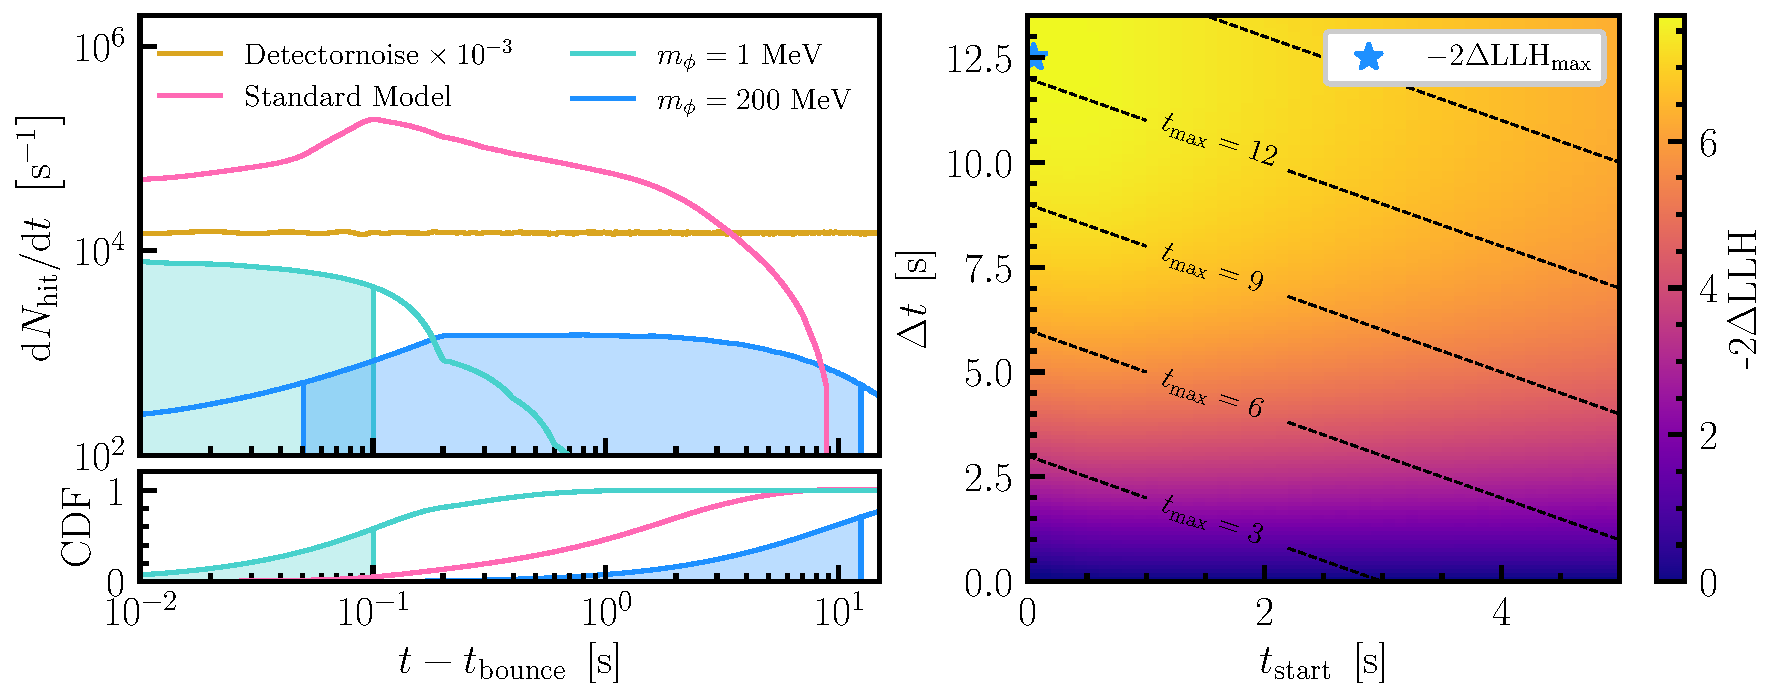
\includegraphics[width=0.95\textwidth]{figures/hits_and_likelihood.pdf}
    \caption{\textbf{\textit{Timing profile of hits and test statistic as a function of the timing window.}}
    In the left panel, we show the hit rate from the SM neutrino flux which peaks at around 0.1~s, coinciding with the peak emission of $\bar{\nu}_{e}$ from the SN. The shaded regions correspond to the timing windows that give peak sensitivity to the particular model. These are the same benchmarks in the parameter space as in \cref{fig:fluxes}.
    In the right panel, we show the test statistic as a function of the starting time and length of the window for the heavy Majoron benchmark ($m_\phi=200$ MeV).
    The relatively broad distribution of high test-statistic values shows that this analysis technique does not require extremely precise reconstruction of the $t_{\mathrm{bounce}}$.
    }
    \label{fig:hits_and_likelihood}
\end{figure*}

We can obtain the flux of daughter $\nu$ by considering decays that occur only at $L_1\geq R^{\nu}_{\rm SN}$.
As the smallest decay distance beyond which the daughter neutrino can escape the explosion unperturbed is roughly the radius of the core, we take $R^{\nu}_{\rm SN} = \unit[30]{km}$.
We will also limit our analysis to a maximal time window of $\unit[100]{s}$ after SN bounce.
This time window is larger than typical values of time delay arising in the model.


As $\bar{\nu}_e$ contribute chiefly to the signals at IceCube via inverse beta decay (IBD), we show in~\cref{fig:fluxes} the differential fluxes of daughter $\bar{\nu}_e$ at different times for two benchmark points in the Majoron model, in comparison to the SM $\bar{\nu}_e$ flux.
We expect the observed signal timing distribution at IceCube to follow these patterns of $\bar{\nu}_{e}$ flux. 

From \cref{fig:fluxes}, we can observe that the energy of $\bar{\nu}_e$ from Majoron decay extends to $\unit[100]{MeV}$ and above for both benchmarks, as expected. 
Consider the light Majoron case in \cref{fig:fluxes}.
Majorons, generating neutrinos with $E_{\bar{\nu}_e} \geq \unit[150]{MeV}$, are nearly relativistic with the emission angle $\alpha$ close to zero.
The time delay can be estimated from the first term in \cref{eq:deltat} given by $\delta t \sim L_\phi (1/\beta -1)\lesssim \unit[0.01]{s}$.
With such a negligible time delay, the time dependence of the $\bar{\nu}_e$ flux is mainly inherited from that of the Majorons upon production, with larger fluxes at $t\leq \unit[0.05]{s}$.
Notice that such a $\bar{\nu}_e$ flux would arrive at the detector earlier than the peak of the SM $\bar{\nu}_e$ flux, which is around $t\simeq \unit[0.1]{s}$ (see \cref{fig:fluxes}), and it potentially leads to early signals at IceCube.
Following \cref{eq:deltat}, the time delay for $\bar{\nu}_e$ with energy $E_{\bar{\nu}_{e}} \sim \unit[10]{MeV}$ is typically $\gtrsim \unit[0.1]{s}$.
These $\bar{\nu}_e$ could be produced from Majorons with low energy of $\mathcal{O}(\unit[10]{MeV})$ or with high energies.
For the low-energy Majoron case, the time delay is mainly due to slow-moving Majorons, while for the high-energy case, it is mainly from the detour.
Such sizable time delays will shift the $\bar{\nu}_e$ peak flux to later times, in comparison to that of their mother Majorons, as exhibited in \cref{fig:fluxes}.



For the heavy Majoron case, the resulting $\bar{\nu}_e$ flux is larger at later times, manifesting the time delay from slowly moving Majorons.
For the heavy Majoron benchmark in \cref{fig:fluxes}, we can estimate that $\delta t \gtrsim \unit[10]{s}$ for $E_{\bar{\nu}_{e}}\sim \unit[200]{MeV}$ which is delayed compared to the peak of the SM $\bar{\nu}_e$ flux.
Compared to the light Majoron case, such a large time delay is a combination of a more slowly moving Majoron and a larger detour due to its large emission angle.

As $L_1\lesssim L_\phi$, the time spread of the flux is roughly given by the aforementioned characteristic value of time delay, which is $\unit[0.1]{s}$ ($\gtrsim\unit[10]{s}$) for the light (heavy) benchmark case.
%%%%%%%%%%%%%%%%%%%%%%%%%%%%%%%%%%%%%%%%%%%%%%%%%%%%%%%%%%%%%%%%%%%%%%%%%%%%%%%%%%%%%%%%%%%%%%%%%%%%%%%%%%%%%


\textbf{\textit{Detector Response and Statistical Treatment}}---The IceCube Neutrino Observatory comprises 5,160 light-detecting digital optical modules (DOMs) buried in a cubic kilometer of the deep, transparent Antarctic ice sheet~\cite{IceCube:2016zyt}.
The DOMs are arranged on 86 strings of 60 DOMs each, with an interstring distance of 125~m (70~m for the eight centermost strings).
These DOMs detect the photons emitted by the charged byproducts of a neutrino interaction in or near the instrumented volume.
This enables IceCube to resolve individual neutrinos with energies ranging between a few GeV and a few PeV.
The neutrinos produced by SNe are far below this threshold and cannot be individually resolved; however, the immense number of neutrinos produced in a SN increases the single-photon rate of the detector.
This dramatic increase in the rate of photons can be distinguished from the background caused by dark noise and radioactive activity in the DOM glass to enable the detection of galactic SN events~\cite{Griswold:2023iwz}.

New physics will affect the development of a SN and distort the temporal structure of the photon signal seen in the IceCube detector.
Thus, one may look for excess events in certain time intervals as evidence of this new physics.
In this work, we simulate the light curve produced by a standard SN with a progenitor mass of $8.8~M_{\odot}$ and those produced by different BSM scenarios mentioned previously; see the left-hand panel of \cref{fig:hits_and_likelihood} for light curves of the same two benchmarks from \cref{fig:fluxes}.

Since more than 93\% of the photons detected in IceCube originate in IBD interactions~\cite{IceCube:2011cwc}, the SM-only event rate peaks at around 0.1~s.
BSM scenarios, on the other hand, can give rise to an early or delayed signal depending on the particulars of the model.
In essence, Majorons can be generated before the peak of the SM $\bar{\nu}_{e}$ flux, and as light Majorons can travel nearly relativistically, they can escape the SNe with negligible time delay and then decay to an all-flavor flux of neutrinos, producing early $\bar{\nu}_{e}$ fluxes before the SM one.
The higher-mass Majorons, on the other hand, acquire a time delay from traveling sub-luminally and at a large detour, thus producing a later signal with sizable time delay.

We use the \texttt{ASTERIA}~\cite{spencer_griswold_2020_3926835} package to simulate the detector response to the different SN scenarios and the thermal and radioactive noise in the DOMs.
This package simulates light yields from coherent $\nu_{e}$ scattering off electrons in the ice, IBD of $\bar{\nu}_{e}$ on nuclei in the ice, and charged- and neutral-current interactions for $\nu_{\alpha}$. In addition to photons produced in neutrino interactions, it also simulates photons from thermal noise in the IceCube photomultipliers (PMTs) and from radioactive decay in the pressure glass housing.
In order to interface with \texttt{ASTERIA}, we use the \texttt{SNEWPY}~\cite{SNEWS:2021ewj} package and, in particular, the \texttt{ParametrizedFlux} object to parametrize the flux with the ``pinching'' factor~\cite{Keil:2002in,SNEWS:2021ewj}.

Since each DOM only sees photons originating from within a sphere of radius $\sim 5.2$~m~\cite{IceCube:2011cwc}, each module can be treated independently if the intermodule spacing is $\gtrsim10.4$~m.
This criteria will be met in IceCube-Gen2~\cite{IceCube-Gen2:2020qha}, and thus, we should expect the total number of hits to scale like the effective photocathode area, \textit{i.e.}:
$$
A_{\mathrm{eff}}^{\mathrm{PC}} = \sum_{i} \varepsilon_{i} A_{i}^{\mathrm{PC}},
$$
where $\varepsilon_{i}$ and $A_{i}^{\mathrm{PC}}$ are the quantum efficiency and photocathode area of a PMT and the sum runs over all PMTs in the detector.
Using this method, we rescale the results from the simulation from IceCube to IceCube-Gen2 in order to estimate IceCube-Gen2's sensitivity.

With the number of hits in the detector from noise, SM-only scenarios, and BSM scenarios as a function of time, we can then quantify the probability of seeing a certain number of hits in a given time window with
\begin{equation}
\label{eq:likelihood}
    -2\Delta\mathrm{LLH} = 2 \left[N_{\mathrm{exp.}} - N_{\mathrm{obs.}} + N_{\mathrm{obs.}}\log\left(\frac{N_{\mathrm{obs.}}}{N_{\mathrm{exp.}}}\right)\right],
    % -2\Delta\mathrm{LLH}(t_{\mathrm{start}}, \Delta t) = 2 \left[N_{\mathrm{exp.}} - N_{\mathrm{obs.}} + N_{\mathrm{obs.}}\log\left(\frac{N_{\mathrm{obs.}}}{N_{\mathrm{exp.}}}\right)\right].
\end{equation}
where $N_{\mathrm{obs.}}$ is the number of photons seen in the detector in the given time and $N_{\mathrm{exp.}}$ is the number of photons expected from a particular BSM hypothesis. 
For each BSM hypothesis, we select the time range that maximizes the test statistic and use that maximal test statistic value.
The optimal ranges for each physics hypothesis are shown by the shaded regions in the left panel of \cref{fig:hits_and_likelihood}, which is around $\unit[0.1]{s}$ ($\unit[10]{s}$) for the light (heavy) benchmark case, consistent with its time spread of the produced $\bar{\nu}_e$ flux.

In the right-hand panel of \cref{fig:hits_and_likelihood}, we show the test statistic as a function of the time at which the time range begins, $t_{\mathrm{start}}$, and the duration of the time range, $\Delta t$, for an example BSM hypothesis. The distribution of test-statistic values is not sharply peaked in time.
Thus, this analysis retains much of its sensitivity even with errors on the reconstruction of $t_{\mathrm{bounce}}\sim\mathcal{O}\left(10^{-3}~\mathrm{s}\right)$~\cite{Halzen_2009}.



%%%%%%%%%%%%%%%%%%%%%%%%%%%%%%%%%%%%%%%%%%%%%%%%%%%%%%%%%%%%%%%%%%%%%%%%%%%%%%%%%%%%%%%%%%%%%%%%%%%%%%%%%%%%%%

\textbf{\textit{Results and Discussions}}---
\begin{figure}[t!]
    \centering
    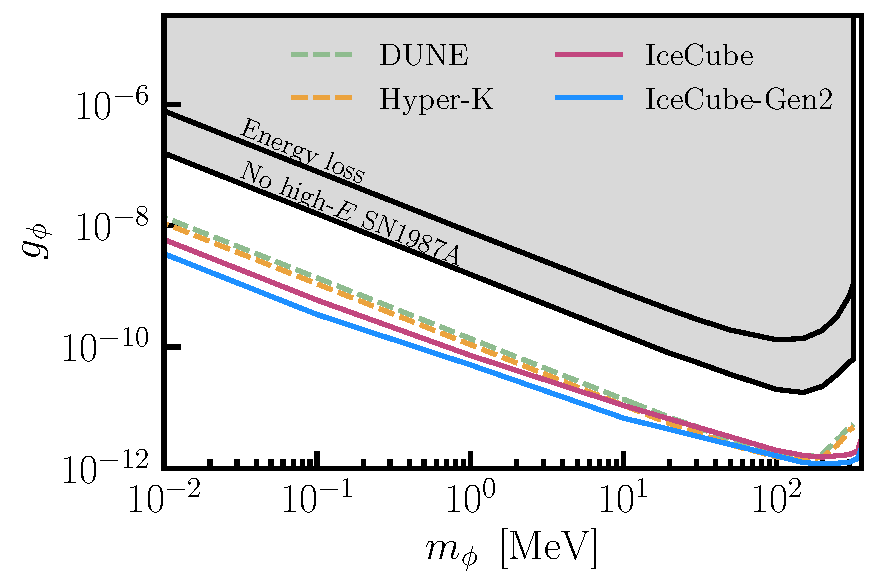
\includegraphics[width=0.47\textwidth]{figures/majoran_sensitivity}
    \caption{\textbf{\textit{Exclusion sensitivities for the Majoron case.}}
    The lines on this plot show the exclusion sensitivity for IceCube, IceCube Gen-2, Hyper-Kamiokande and DUNE at $2\sigma$ CL.
    Additionally, we also show the reaches by SN cooling and by the lack of observation of high-energy neutrinos from SN1987A as black lines. 
    The sensitivities shown by the dashed line are obtained following~\cite{Brdar:2023tmi} with time-integrated data.
    }
    \label{fig:sensitivity}
\end{figure} 
Assuming that IceCube does not observe an excess neutrino above the expected detector backgrounds and SM neutrinos, we obtain the expected $2\sigma$ exclusion limits by finding the coupling where \cref{eq:likelihood} is equal to 3.841.
We show these in \cref{fig:sensitivity} for the Majoron case considering both IceCube and IceCube-Gen2.
To illustrate the broad physics application of the analysis, we also show results for the sterile neutrino case with magnetic portal in the Supplemental Materials.
Current limits~\cite{Fiorillo:2022cdq} from the energy loss requirement, and non-observation of high-energy SN neutrinos from SN 1987A are also shown in \cref{fig:sensitivity} for the Majoron case.
A future SN explosions would enable IceCube to improve current limits by one order of magnitude. 
Moreover, while current limits from time-integrated observables follow the behavior of $g_\phi\propto m^{-1}_\phi$ as Majoron production rate is proportional to $(g_\phi m_\phi)^2$, IceCube can provide a stronger limit than this by focusing on the time window, especially before the peak of SM $\bar{\nu}_e$ fluxes, to reduce SM condemnations.

We also present the estimated reaches of DUNE and Hyper-Kamiokande in \cref{fig:sensitivity} by looking for time-integrated high-energy neutrinos following Refs.~\cite{Fiorillo:2022cdq, Brdar:2023tmi}.
While the constraints from IceCube for the intermediate mass region are comparable to that from DUNE and Hyper-Kamiokande, we observe that for both low-mass region $m_\phi \lesssim \unit[10]{MeV}$ and high-mass region $m_\phi \gtrsim \unit[200]{MeV}$, IceCube can provide stronger constraints.
This is the outcome we expect.
For light $\phi$ case with negligible time delay, IceCube would observe early signals in a time window separated from that when most of the SM flux contribution appears, as we show in the left panel of \cref{fig:hits_and_likelihood}, thus enhancing the reaches. On the high mass end, neutrino signals will arrive much later than the SM case, where a time window at late time can be considered to reduce the standard neutrino contamination. 

There are existing uncertainties from different modeling of SN explosions (see e.g. Ref.~\cite{li2023old}) as well as discrepancies between SN 1987A neutrino data and modeling. Nevertheless, we point out that even the uncertainties of around $2\sigma$  will only change our exclusion limits by a small factor.
We make the code used in this work publicly available so that the impact of SN modeling uncertainties on the sensitivity of neutrino telescopes to BSM scenarios can be further explored.

\textbf{\textit{Summary}}---
In this Letter, we have demonstrated that neutrino telescopes such as IceCube can provide unprecedented probes of new physics, such as Majoron-like bosons and neutrino magnetic moment portal, by measuring SN time profiles to a window as short as $\mathcal{O}(0.01)$ s. Specifically, signatures outside the SM neutrino time window, including both early and delayed signals, can be effectively probed by neutrino telescopes. This analysis can be extended to test other BSM realizations including, but not limited to, sterile neutrinos with a mixing portal.
Additionally, the code used to probe these models is publicly available on \href{https://github.com/jlazar17/NuTel_SNe_BSM/}{GitHub}.
%%%%%%%%%%%%%%%%%%%%%%%%%%%%%%%%%%%%%%%%%%%%%%%%%%%%%%%%%%%%%%%%%%%%%%%%%%%%%%%%%%%%%%%%%%%%%%%%%%%%%%%%%%%%%

\textit{Acknowledgements}---We want to thank Thomas Janka and Daniel Kresse for providing the data from Garching supernovae simulations---available at \url{https://wwwmpa.mpa-garching.mpg.de/ccsnarchive/} in machine-readable form---and also for stimulating discussions.
We also thank Jackapan Pairin for their help designing figures in this work.
Y.-Y. L is supported by the NSF of China through Grant No. 12305107, 12247103.
CAA are supported by the Faculty of Arts and Sciences of Harvard University, the National Science Foundation (NSF), the NSF AI Institute for Artificial Intelligence and Fundamental Interactions, the Research Corporation for Science Advancement, 
and the David \& Lucile Packard Foundation.
CAA and JL were partially supported by the Alfred P. Sloan Foundation for part of this work.
JL is supported by the Belgian American Educational Foundation.


%%%%%%%%%%%%%%%%%%%%%%%%%%%%%%%%%%%%%%%%%%%%%%%%%%%%%%%%%%%%%%%%%%%%%%%%%%%%%%%%%%%%%%%%%%%%%%%%%%%%%%%%%%



\bibliography{ic_sn_hnl}





\newpage
\onecolumngrid
\appendix

\ifx \standalonesupplemental\undefined
\setcounter{page}{1}
\setcounter{figure}{0}
\setcounter{table}{0}
\setcounter{equation}{0}
\fi

\renewcommand{\thepage}{Supplemental Methods and Tables -- S\arabic{page}}
\renewcommand{\figurename}{SUPPL. FIG.}
\renewcommand{\tablename}{SUPPL. TABLE}

\renewcommand{\theequation}{A\arabic{equation}}

\section{Supplemental Methods and Tables}

\section{Appendix A: Dipole Magnetic Moment Portal}
\begin{figure}[hb!]
    \centering
    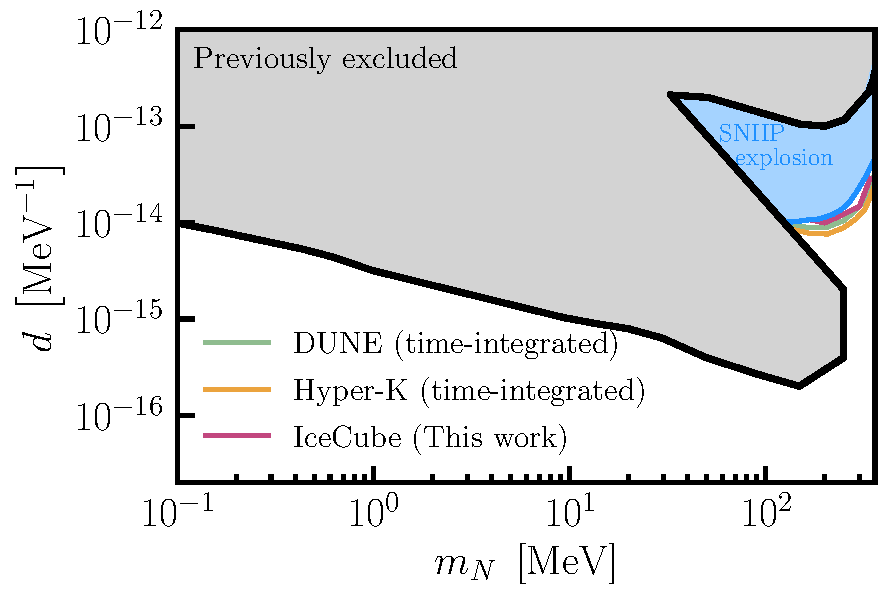
\includegraphics[width=0.47\textwidth]{figures/magnetic_moment_sensitivity}
    \caption{\textbf{\textit{Exclusion sensitivities for the magnetic moment case.}}
    The lines on this plot show the exclusion sensitivity for IceCube, IceCube-Gen2, and the limits computed in~\cite{Brdar:2023tmi} for Hyper-Kamiokande and DUNE. 
    The sensitivities shown by the dashed line have been previously computed~\cite{Brdar:2023tmi} and use time-integrated data.
    %Sensitivities indicated by solid lines are newly computed in this work, whereas those shown by dashed lines have been previously computed in~\cite{Brdar:2023tmi}
    The shaded regions are excluded by the combination of energy loss requirement, non-observation of photon and neutrino signals from SN1987A studied in~\cite{Brdar:2023tmi} and by constraints on the energy release from SN explosion (SNIIP explosion)~\cite{PhysRevLett.128.221103, chauhan2024probing}.
    }
    \label{fig:magnetic_moment_sensitivity}
\end{figure}
Here we also present results for active-to-sterile neutrino transition magnetic moment described by~\cite{Magill:2018jla,Brdar:2020quo,Brdar:2023tmi}
\begin{align}
    \mathcal{L} \supset \sum_\alpha d_\alpha \bar{N}\sigma_{\mu\nu} \nu^{\alpha} F^{\mu\nu}-\frac{M_N}{2} \bar{N}^c N + \text{h.c.}\,,
    \label{eq:Lag}
\end{align}
where $\nu^{\alpha}$ and $N$ represent active and sterile neutrinos, respectively. Further, $F^{\mu\nu}$ is the field strength tensor of the electromagnetic field, $d_\alpha$ is the dimensionful coefficient of this dimension-5 term and $M_N$ is sterile neutrino mass.  We assume flavor universal interaction $d_\alpha \equiv d$. We consider the two production channels for $N$ inside the SN: $\nu e^- \to N e^-$ at lower energies and $\nu \gamma \to N$ for larger active neutrino energies. Both processes occur due to the interaction term in \cref{eq:Lag}; after $N$ are produced, they decay to active neutrinos and photons which is again realized through the same term in the Lagrangian, with the decay width for $N\to\nu\gamma$ given by $\Gamma_N = 6d^2 M_N^3/4 \pi$~\cite{Plestid:2020vqf}. The limits from IceCube are shown in SUPPL. \cref{fig:magnetic_moment_sensitivity}, together with previously excluded regions by energy loss, non-observations of photons and neutrinos from SN1987A~\cite{Brdar:2023tmi}, and constraints on the energy release from low-energy SN explosions (SNIIP)~\cite{PhysRevLett.128.221103, chauhan2024probing}. We also point out that by neglecting the $N$ production channel $\nu p^+\to N p^+$ inside SN, the limits we obtained are conservative relative to the SNIIP region taken from~\cite{chauhan2024probing}. We notice that the time delay near the exclusion boundary is typically of $\Delta t \sim \mathcal{O}(1)$ sec, which is longer than the standard $\bar{\nu}_e$ peak luminosity time scale and this is why IceCube does not improve over the limits computed in~\cite{Brdar:2023tmi} for DUNE and Hyper-Kamiokande. 

\end{document}

